\documentclass[11pt]{article}  
\usepackage[margin=1in]{geometry}
\parindent=0in
\parskip=8pt
\usepackage{fancyhdr,amssymb,amsmath, graphicx, listings,float,subfig,enumerate,epstopdf,color,multirow,setspace,bm,textcomp}
\usepackage[usenames,dvipsnames]{xcolor}
\usepackage{hyperref}
\usepackage{graphicx}
\usepackage[utf8]{inputenc}
\usepackage{amsmath}
\graphicspath{{./Images}}

\pagestyle{fancy}


\begin{document} 

\lhead{Assignment \# 2}
\chead{Robert Denim Horton}
\rhead{\today}

\begin{center}\begin{Large}
CS 4720/5720 Design and Analysis of Algorithms

Homework \#2

Student: (Robert Denim Horton)
\end{Large}
\end{center}


\section*{Answers to homework problems:}

\begin{enumerate}
	% Question 1
	\item Consider the following graphs in Figure 1.1
	\begin{center}
		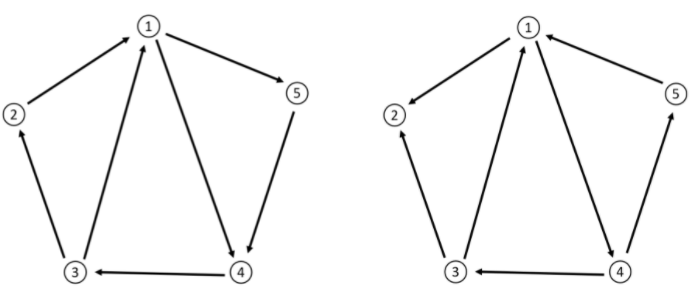
\includegraphics[scale=0.6]{Question1_Figure1.1}\\
		Figure 1.1
	\end{center}
		\begin{enumerate}[(a)]
			% Question 1: Part 1
			\item Are these graphs strongly connected? Explain why or why not.
			% Question 1: Part 2
			\item Are these graphs aperiodic? If a graph is periodic, compute its period.
		\end{enumerate}
\end{enumerate}
\textcolor{gray}{
Answers:
\begin{enumerate}
	\item Consider the following graphs in Figure 1.1
	\begin{enumerate}[a]
		% Question 1: Part 1
		\item In Figure 1.1 we see two different directed graphs.  To check if a graph is strongly connected or not a \textit{depth first search} can be done on the graph starting from some node, $x_i$, in set, $X$, of nodes that exists in the graph $G$.  The depth search is a pretty common algorithm the steps through the graph trying to visiting each pair of nodes through the edges that exist. If there exists a path in between any pair of nodes we call the graph strongly connected.  As we can see looking at the graph on the left that there exists a path in-between all the nodes that traverses along the outside of the graph. So we can say that this graph is strongly connected.  As for the graph on the left we see that node 2 is only visited and has no edges leaving it so their fore any pair of nodes that is looking for a path from node 2 to other node does not exsist and we can call this graph weakly connected. 
		% Question 1: Part 2
		\item As for checking if the two graphs in Figure 1.1 are aperiodic or not, in mathematical areas of graph theory, directed graphs are said to be aperiodic if there is no integer, $k$, that is grater than 1 that divides the length of every cycle of the graph.  This is to say that for the matrix made up for the graph on the left,
		$$\begin{bmatrix} 
			0 & 0 & 0 & 1 & 1 \\
			1 & 0 & 0 & 0 & 0 \\
			1 & 1 & 0 & 0 & 0 \\
			0 & 0 & 1 & 0 & 0 \\
			0 & 0 & 0 & 1 & 0
		\end{bmatrix},$$
we can call it periodic 
		$$\begin{bmatrix} 
			0 & 1 & 0 & 1 & 0 \\
			0 & 0 & 0 & 0 & 0 \\
			1 & 1 & 0 & 0 & 0 \\
			0 & 0 & 1 & 0 & 1 \\
			1 & 0 & 0 & 0 & 0 \\
		\end{bmatrix}$$
	\end{enumerate}
\end{enumerate}
}

% Question 2
\begin{enumerate}
	\setcounter{enumi}{1}
	\item Consider the following weighted adjacency matrix in Figure 1.2:
	\begin{center}
		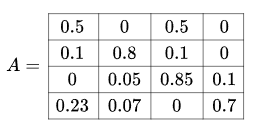
\includegraphics[scale=0.6]{Question2_Figure1.2}\\
		Figure 1.2
	\end{center}
	\begin{enumerate}[(a)]
		% Question 2: Part 1
		\item Is this matrix row-stochastic?
		% Question 2: Part 2
		\item Draw the graph corresponding to this matrix.
		% Question 2: Part 3
		\item Is the graph strongly connected?
		% Question 2: Part 4
		\item Is the graph aperiodic?
	\end{enumerate}
\end{enumerate}
\textcolor{gray}{
Answers:
\begin{enumerate}
	\setcounter{enumi}{1}
	\item Consider the following weighted adjacency matrix in Figure 1.2:
	\begin{enumerate}[a]
			% Question 2: Part 1
			\item Is this matrix row-stochastic?
			% Question 2: Part 2
			\item Draw the graph corresponding to this matrix.
			% Question 2: Part 3
			\item Is the graph strongly connected?
			% Question 2: Part 4
			\item Is the graph aperiodic?
	\end{enumerate}
\end{enumerate}
}

\begin{enumerate}
	\setcounter{enumi}{2}
	% Question 3
	\item Consider the following graph in Figure 1.3
	\begin{center}
		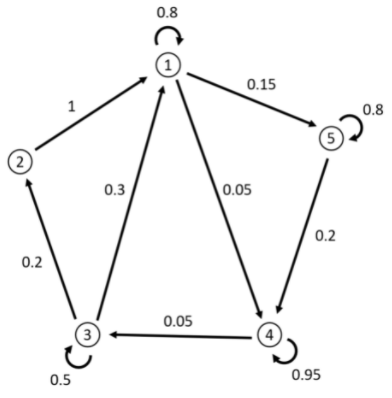
\includegraphics[scale=0.6]{Question3_Figure1.3}\\
		Figure 1.3
	\end{center}
	\begin{enumerate}[(a)]
		% Question 3: Part 1
		\item Write the weighted adjacency matrix corresponding to this graph. Verify that the graph you wrote is row-stochastic.
		% Question 3: Part 2
		\item By hand, using matrix multiplication, perform 1 step of the DeGroot opinion dynamic model on this graph with initial opinions of (1, 1, 0.5, 0, 0).
		% Question 3: Part 3
		\item In the DeGroot opinion dynamics model, which node's initial opinion gets the most weight in society's final opinion? Which node gets the least weight? (it is highly recommended that you use computer code to answer this question).
	\end{enumerate}	
\end{enumerate}
\textcolor{gray}{
Answers:
\begin{enumerate}
	\setcounter{enumi}{2}
	% Question 3
	\item Consider the following graph in Figure 1.3
	\begin{enumerate}[(a)]
		% Question 3: Part 1
		\item Write the weighted adjacency matrix corresponding to this graph. Verify that the graph you wrote is row-stochastic.
		% Question 3: Part 2
		\item By hand, using matrix multiplication, perform 1 step of the DeGroot opinion dynamic model on this graph with initial opinions of (1, 1, 0.5, 0, 0).
		% Question 3: Part 3
		\item In the DeGroot opinion dynamics model, which node's initial opinion gets the most weight in society's final opinion? Which node gets the least weight? (it is highly recommended that you use computer code to answer this question).
	\end{enumerate}	
\end{enumerate}
}

% Question 4
\begin{enumerate}
	\item Consider again the graph from problem 2 (Figure 1.2).
	\begin{enumerate}[(a)]
		% Question 4: Part 1
		\item By hand, using matrix multiplication, perform 1 step of the Friedkin-Johnsen opnion dynamic model on this graph with initial opinions of (1, 1, 0.5, 0, 0) and lambda values of (0.9, 0.1, 0.8, 1, 0.5).
		% Question 4: Part 2
		\item As we discussed in class, in the Friedkin-Johnsen model, nodes usually have differing opinions even after a long time. Keeping the lambda values from part A, experiment with this graph and try to find an assignment of initial opinions that results in the most different limiting opinions. That is, what equilibrium on this graph can have the most disagreement out of all equilibria? You will likely want to use compute code to solve this problem. Full credit is possible if you show understanding and effort; I will award 1 bonus point if you can show that your answer is the most disagreement possible.
	\end{enumerate}
\end{enumerate}
\textcolor{gray}{
Answers:
\begin{enumerate}
	\setcounter{enumi}{3}
	\item Consider again the graph from problem 2 (Figure 1.2).
	\begin{enumerate}[(a)]
		% Question 4: Part 1
		\item By hand, using matrix multiplication, perform 1 step of the Friedkin-Johnsen opnion dynamic model on this graph with initial opinions of (1, 1, 0.5, 0, 0) and lambda values of (0.9, 0.1, 0.8, 1, 0.5).
		% Question 4: Part 2
		\item As we discussed in class, in the Friedkin-Johnsen model, nodes usually have differing opinions even after a long time. Keeping the lambda values from part A, experiment with this graph and try to find an assignment of initial opinions that results in the most different limiting opinions. That is, what equilibrium on this graph can have the most disagreement out of all equilibria? You will likely want to use compute code to solve this problem. Full credit is possible if you show understanding and effort; I will award 1 bonus point if you can show that your answer is the most disagreement possible.
	\end{enumerate}
\end{enumerate}
}
\end{document}
